\subsection*{Pertanyaan: Analisis graf pada Gambar 7.5 dan tuliskan satu cara urutan pewarnaan simpul secara manual dengan algoritma Backtracking apabila menggunakan 3 warna: merah, hijau, dan biru!}

\textbf{Graf Gambar 7.5:} Graf terdiri dari 5 simpul, yaitu 0, 1, 2, 3, dan 4. Edge yang terbentuk adalah 3--4, 3--0, 4--1, 0--1, 0--2, dan 1--2. Karena graf tidak berarah, setiap sisi menunjukkan hubungan dua arah antar simpul.

\begin{figure}[H]
    \centering
    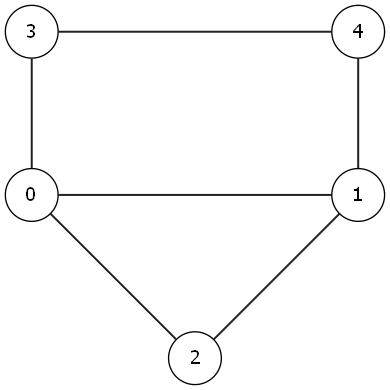
\includegraphics[width=0.5\textwidth]{figures/praktikum7/graf_pretest_75.png}
    \caption{Visualisasi Graf Pre Test dan Post Test Praktikum 7}
    \label{fig:praktikum7-graf-pretest}
\end{figure}

\textbf{Aturan pewarnaan:} Dua simpul yang bertetangga tidak boleh memiliki warna yang sama. Warna yang digunakan adalah merah, hijau, dan biru. Urutan pewarnaan dilakukan dari simpul 0 sampai simpul 4.

\textbf{Daftar ketetanggaan graf:}
\begin{itemize}
    \item Simpul 0 bertetangga dengan simpul 3, 1, dan 2.
    \item Simpul 1 bertetangga dengan simpul 4, 0, dan 2.
    \item Simpul 2 bertetangga dengan simpul 0 dan 1.
    \item Simpul 3 bertetangga dengan simpul 4 dan 0.
    \item Simpul 4 bertetangga dengan simpul 3 dan 1.
\end{itemize}

\textbf{Jawaban manual:}

\begin{table}[H]
    \centering
    \caption{Penelusuran Pewarnaan Graf Manual dengan Backtracking}
    \label{tab:praktikum7-pretest-manual}
    \begin{tabular}{cllp{6cm}}
    \toprule
    \textbf{Langkah} & \textbf{Simpul} & \textbf{Warna} & \textbf{Alasan} \\ \midrule
    1 & 0 & Merah & Simpul 0 diproses pertama, sehingga belum ada tetangga yang membatasi pilihan warna. \\
    2 & 1 & Hijau & Simpul 1 bertetangga dengan simpul 0 yang sudah berwarna merah, sehingga warna merah tidak dapat dipakai. \\
    3 & 2 & Biru & Simpul 2 bertetangga dengan simpul 0 merah dan simpul 1 hijau, sehingga warna aman berikutnya adalah biru. \\
    4 & 3 & Hijau & Simpul 3 bertetangga dengan simpul 0 merah. Warna hijau masih aman karena simpul 4 belum diwarnai. \\
    5 & 4 & Merah & Simpul 4 bertetangga dengan simpul 3 hijau dan simpul 1 hijau, sehingga warna merah dapat digunakan. \\ \bottomrule
    \end{tabular}
\end{table}

Solusi pewarnaan yang diperoleh adalah:
\[
    [1, 2, 3, 2, 1]
\]
Artinya simpul 0 = merah, simpul 1 = hijau, simpul 2 = biru, simpul 3 = hijau, dan simpul 4 = merah.

Solusi tersebut valid karena setiap pasangan simpul yang terhubung oleh edge memiliki warna berbeda. Edge 0--1, 0--2, 0--3, 1--2, 1--4, dan 3--4 semuanya memenuhi aturan pewarnaan graf.

\begin{figure}[H]
    \centering
    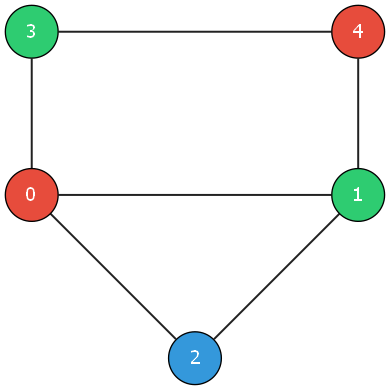
\includegraphics[width=0.5\textwidth]{figures/praktikum7/graf_pretest_75_berwarna.png}
    \caption{Solusi Pewarnaan Manual pada Graf Gambar 7.5}
    \label{fig:praktikum7-graf-pretest-berwarna}
\end{figure}
